\chapter{実機実験}\label{chap:practical_experiment}

\section{はじめに}

\section{環境}

\subsection{開発環境}

\begin{center}
  \begin{tabular}{l|c} 
    \thline
    ノートPC&\\
    \hline
    CPU & 87  \\
    GPU & 72   \\
    RAM & 53   \\
    OS & Ubuntu 18.04 LTS   \\
    ROS Distributions & melodic   \\ 
    \thline
  \end{tabular}
\end{center}


\subsection{実環境}

提案したアルゴリズムを評価するために、図\ref{fig:real_environment}のように、
シミュレータと同じような環境を用意した。実験に使用するロボットとして、図\ref{fig:raspicat}の
既製品の小型移動ロボットであるRaspberry Pi Catを使用した。


\begin{figure}[H]
  \begin{center}
    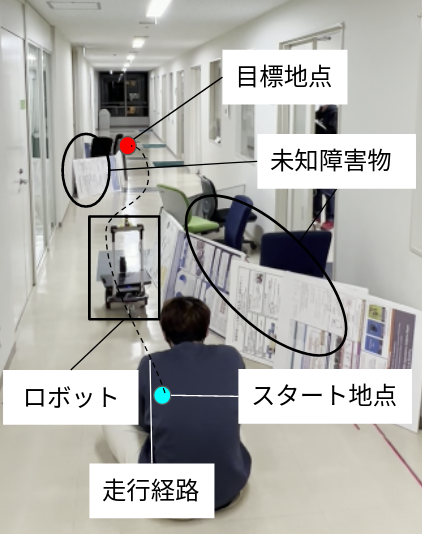
\includegraphics[width=0.5\linewidth]{figs/real_environment.png}
    \caption{実環境とロボット}
    \label{fig:real_environment}
  \end{center}
\end{figure}

\section{実験方法}

図\ref{fig:real_environment}の実環境にて、提案したアルゴリズムを実装したemclの評価を行う。
実験では未知障害物が存在する環境を走行した場合において、以下の項目について評価を行う。
\begin{itemize}
  \item 走行の評価
  \item 自己位置の尤度
  \item 使用された観測パターン
  \item 尤度計算にかかった時間
\end{itemize}
5.3.1では提案した手法の実装がない、5.3.2では提案した手法の実装がある場合において、
自律走行をした際の評価をまとめる。

\subsection{提案した手法の実装無し}

図\ref{fig:nav_no_imp_real}のように、未知障害物が存在する実環境において、
提案した手法の実装が無いリセット付きの自己位置推定の場合、
目標地点にたどり着くことができなかった。これは、手前にある未知障害物によって、リセットがかかり続けたため、
自己位置推定が破綻してしまったことが原因である。

\begin{figure}[H]
  \begin{center}
    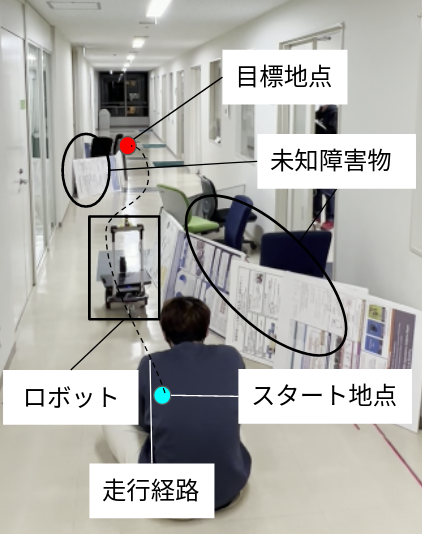
\includegraphics[width=0.5\linewidth]{figs/real_environment.png}
    \caption{自律走行時の自己位置の尤度}
    \label{fig:nav_no_imp_real}
  \end{center}
\end{figure}

自律走行時の尤度は、図\ref{fig:nav_likelihood_no_imp_real}のようになった。
未知障害物付近を走行している5秒辺りでは、尤度が著しく低下してしまっている。
また、未知障害物によってリセットがかかり続け、自己位置推定が破綻してしまったため、15秒までのグラフとなっている。

\begin{figure}[H]
  \begin{center}
    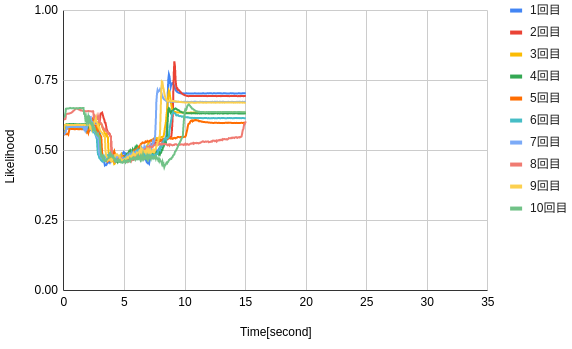
\includegraphics[width=0.98\linewidth]{figs/real_likelihood_before.png}
    \caption{使用したシミュレータ環境とロボット}
    \label{fig:nav_likelihood_no_imp_real}
  \end{center}
\end{figure}

\subsection{提案した手法の実装あり}

提案した手法の実装があるリセット付きの自己位置推定では、目標地点に到達することができた。

\begin{figure}[H]
  \begin{center}
    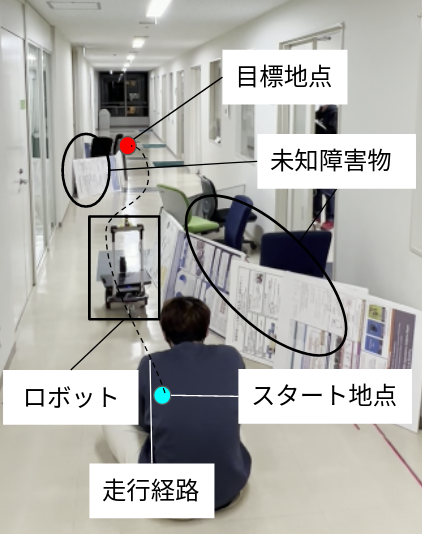
\includegraphics[width=0.5\linewidth]{figs/real_environment.png}
    \caption{自律走行時の自己位置の尤度}
    \label{fig:nav_imp_real}
  \end{center}
\end{figure}

自律走行時の尤度は、図\ref{fig:nav_likelihood_no_imp_real}のようになった。
手前の未知障害物付近の走行時の尤度は安定していたが、
奥側の未知障害物付近の走行時の尤度は著しく低下してしまっている。
しかし、いずれの場合において、高い尤度を保っていることがわかる。

\begin{figure}[H]
  \begin{center}
    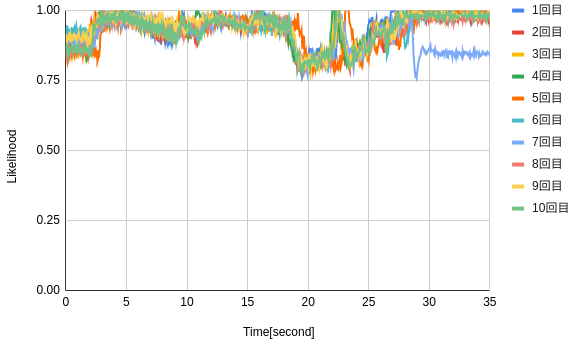
\includegraphics[width=0.98\linewidth]{figs/real_likelihood_after.png}
    \caption{自律走行時の自己位置の尤度}
    \label{fig:sim_world}
  \end{center}
\end{figure}

自律走行時において、パーティクルの中で最も使用された観測パターンを表したグラフは
図\ref{fig:obs_pattern_sim_real}のようになった。
実機での実験結果では、シミュレータでの実験結果である図\ref{fig:obs_pattern_sim}と違い、
パーティクルが様々な観測パターンを選択していることがわかる。

\begin{figure}[H]
  \begin{center}
    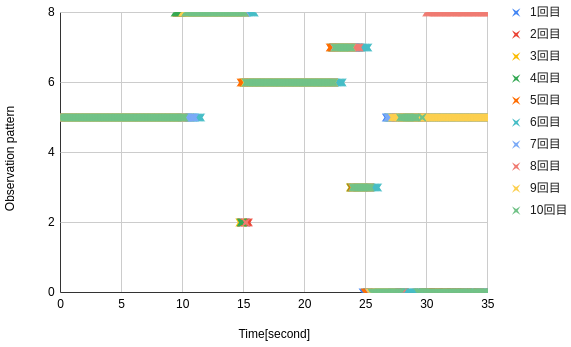
\includegraphics[width=0.98\linewidth]{figs/real_imp_ob_pattern.png}
    \caption{自律走行時にパーティクルの中で最も使用された観測パターン}
    \label{fig:obs_pattern_sim_real}
  \end{center}
\end{figure}
